\subsection{Profile Setup}

\subsubsection{UI Mockup}

\begin{figure}[H]
\centering
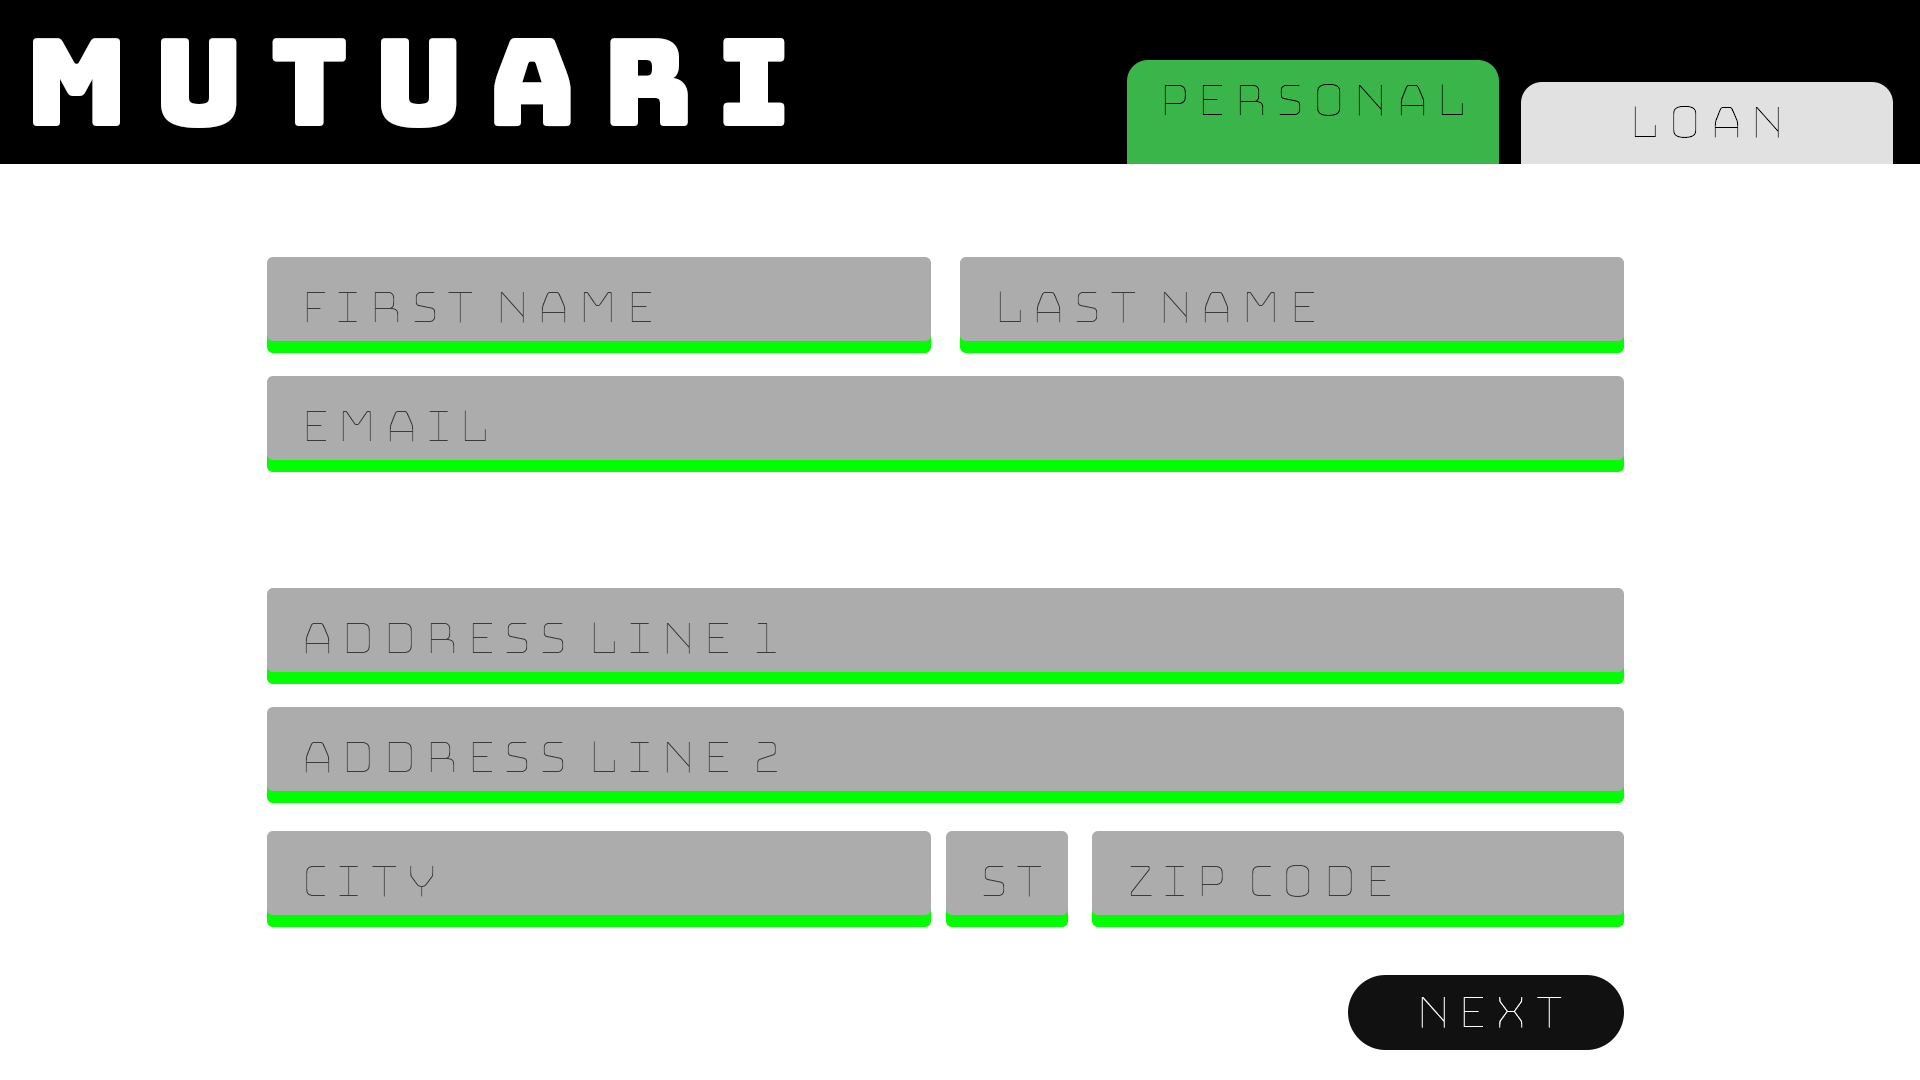
\includegraphics[width=\textwidth]{Account_Creation_Borrower}
\caption{Borrower Signup}
\end{figure}

\begin{figure}[H]
\centering
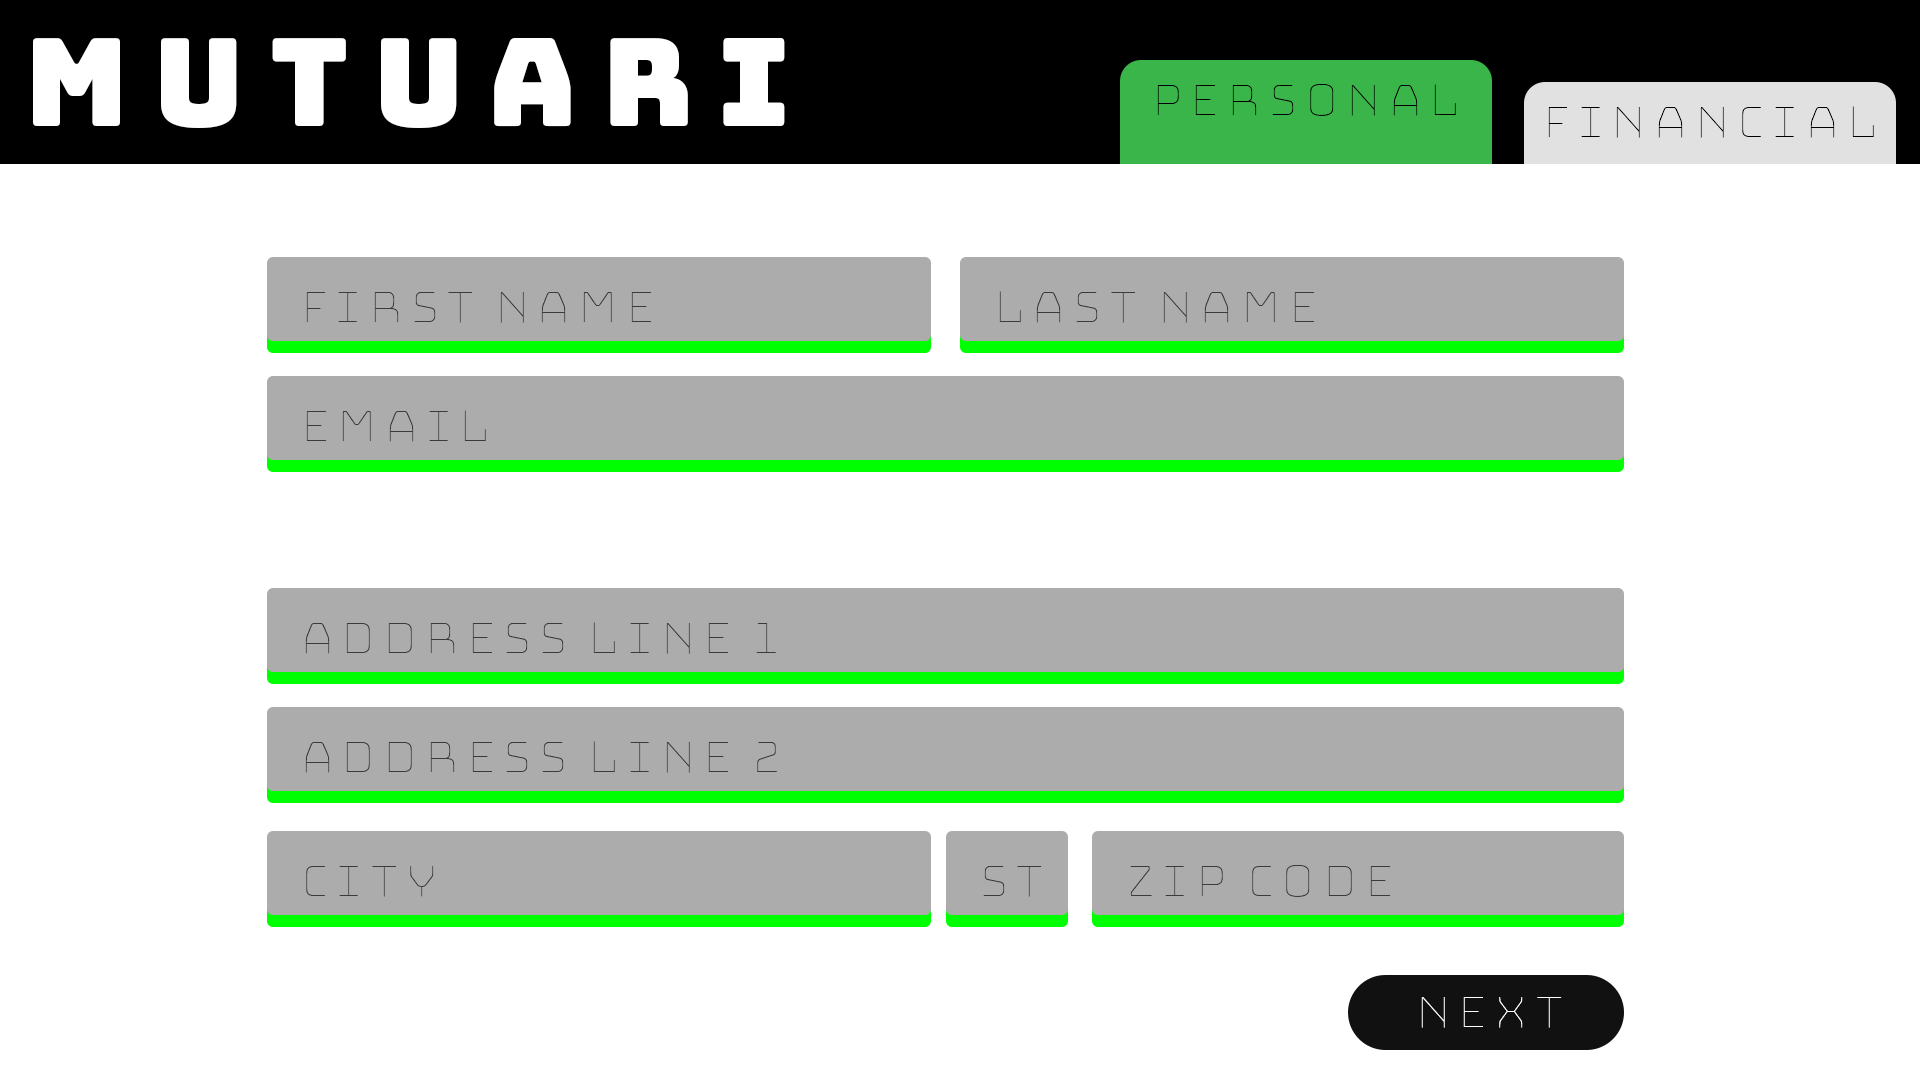
\includegraphics[width=\textwidth]{Account_Creation_Lender}
\caption{Lender Signup}
\end{figure}

\begin{figure}[H]
\centering
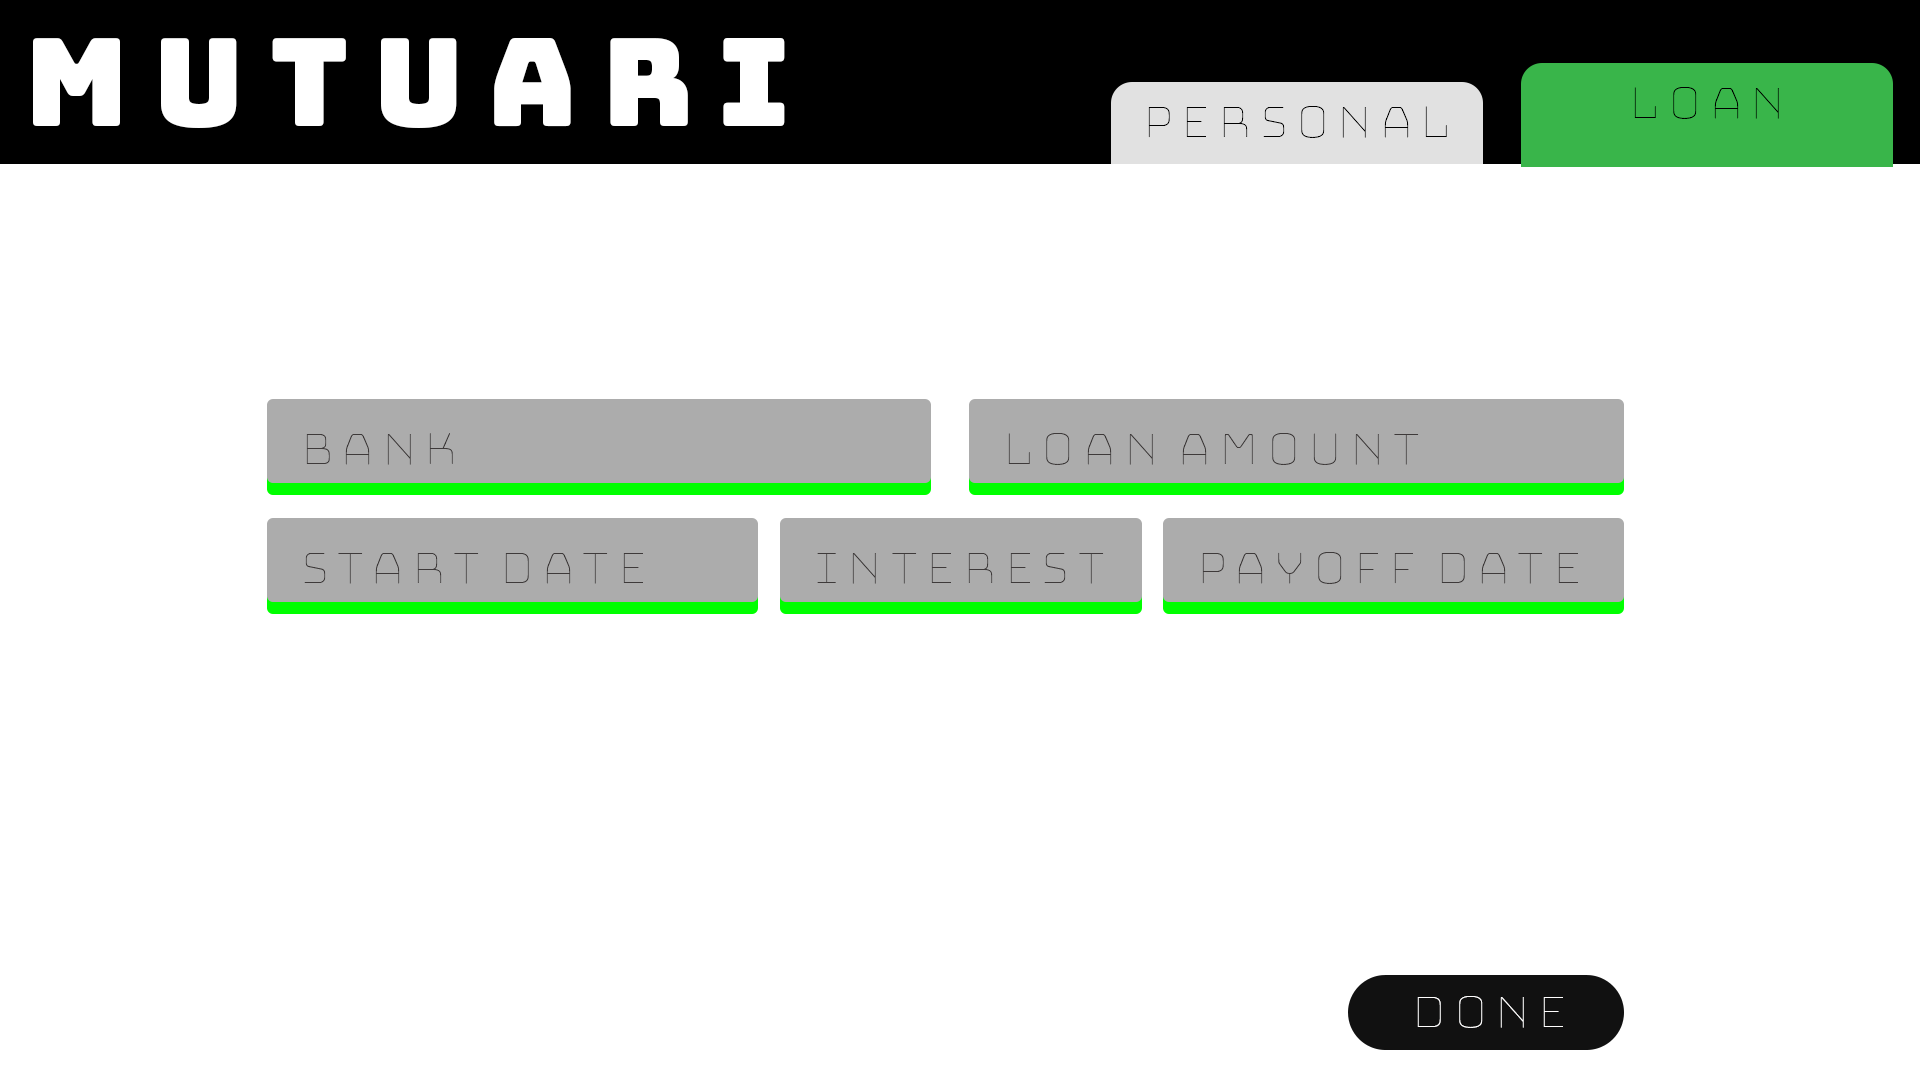
\includegraphics[width=\textwidth]{Account_Creation_Loan_Borrower}
\caption{Borrower Loan information}
\end{figure}

\begin{figure}[H]
\centering
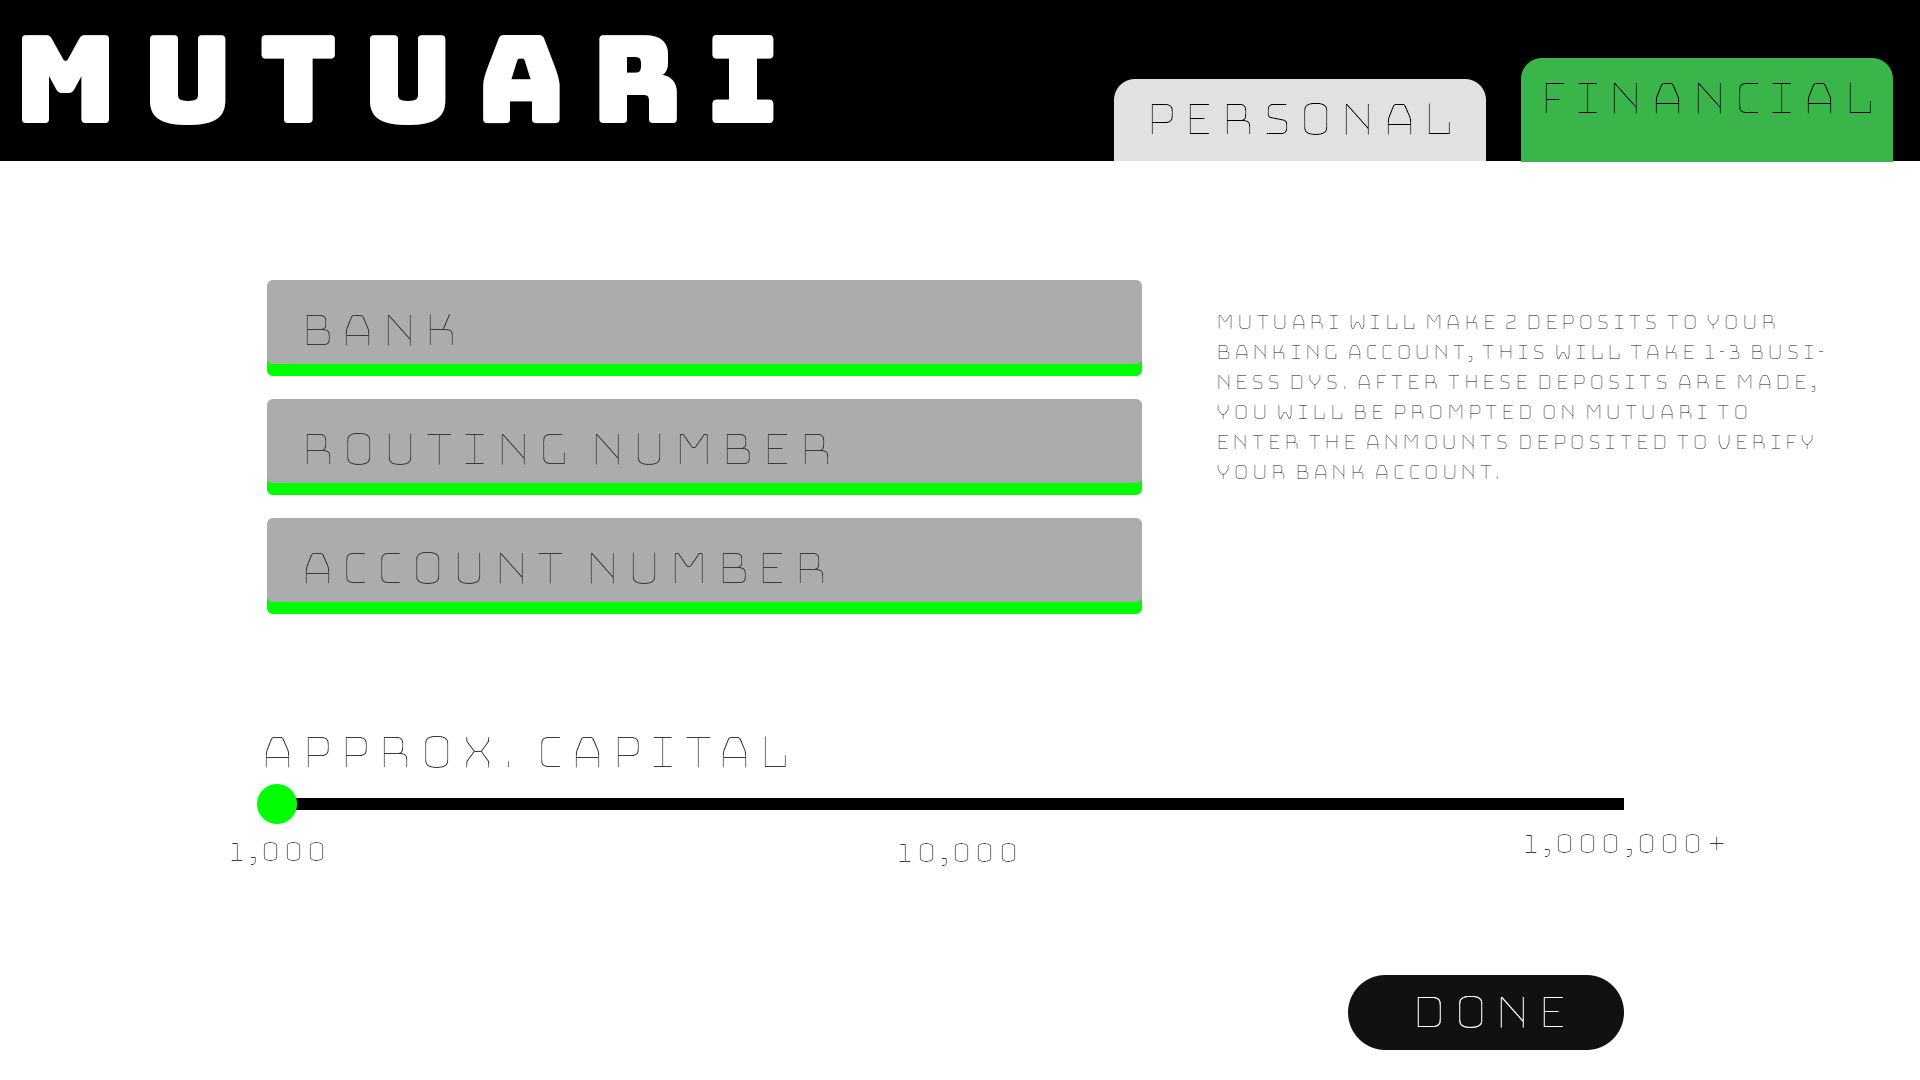
\includegraphics[width=\textwidth]{Account_Creation_Financial_Lender}
\caption{Lender Banking information}
\end{figure}

\begin{figure}[H]
\centering
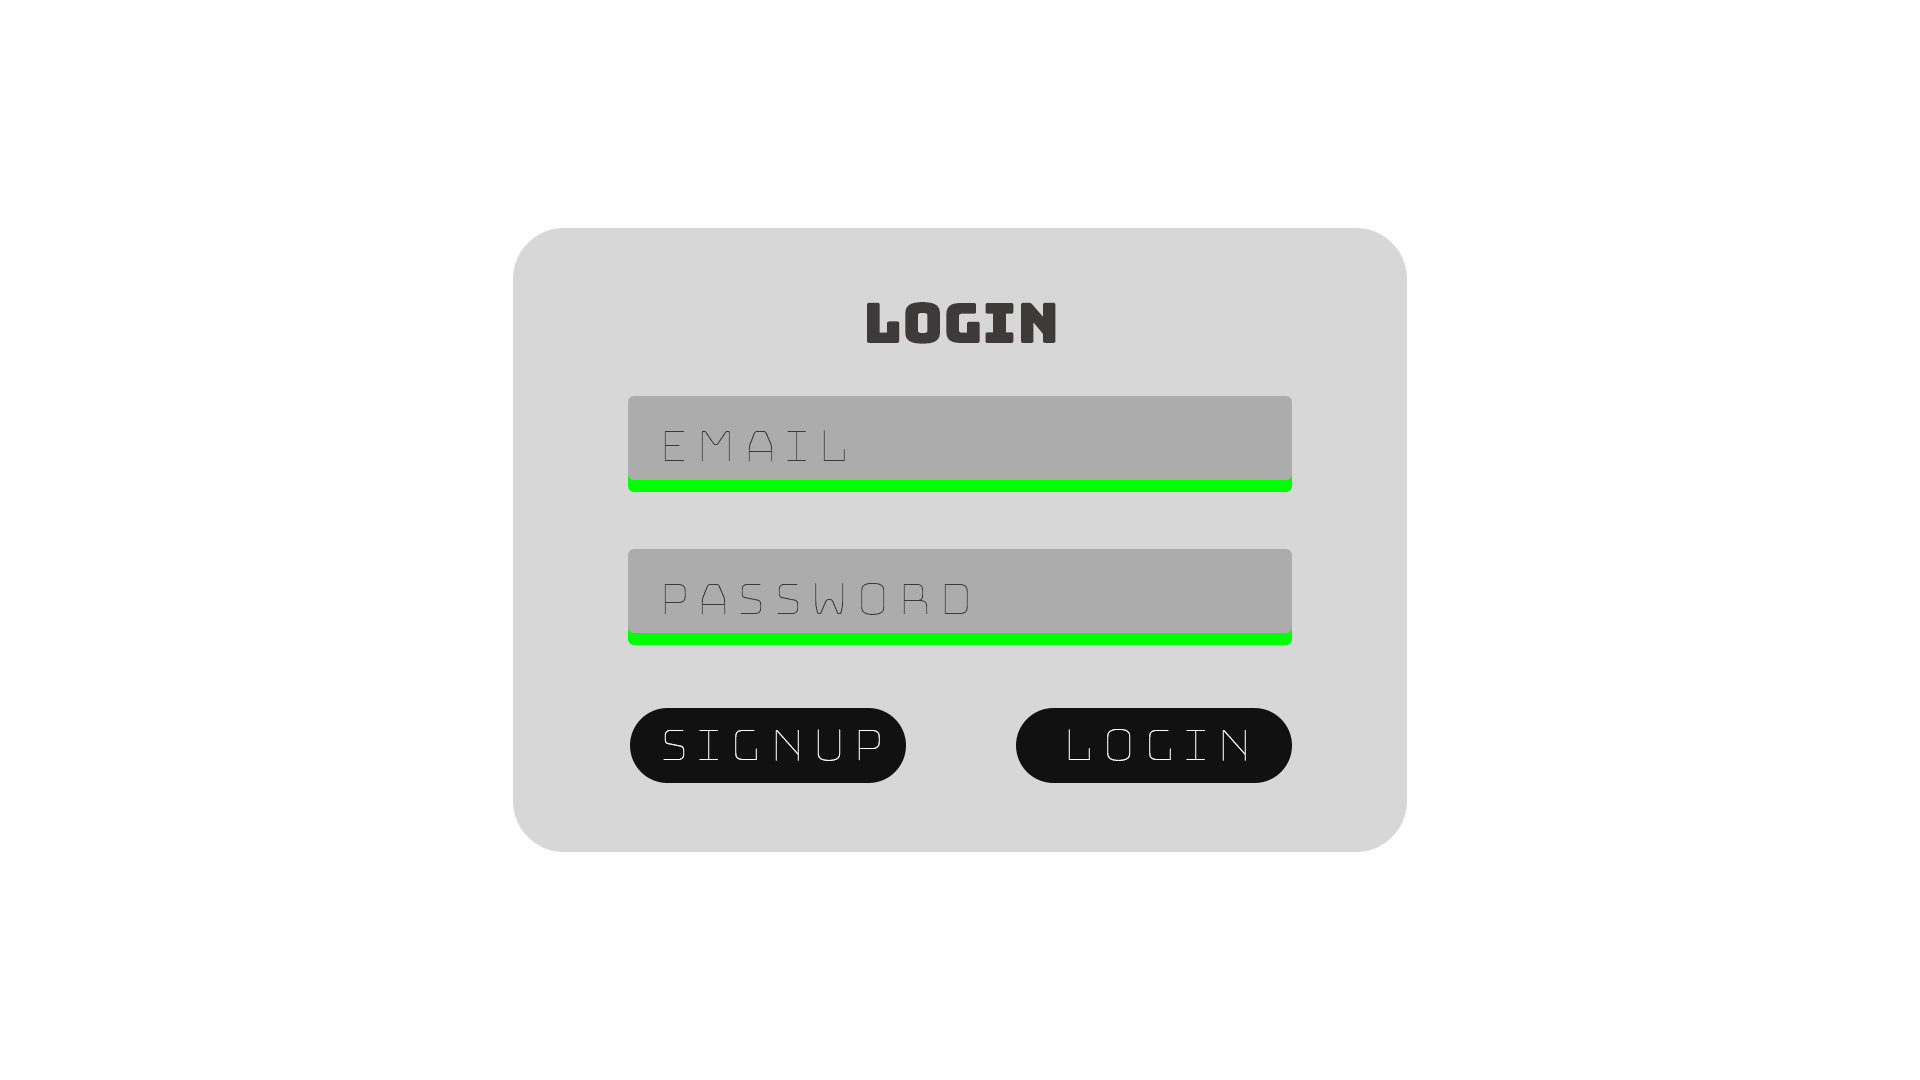
\includegraphics[width=\textwidth]{login_modal}
\caption{Email and Password submission}
\end{figure}

\begin{figure}[H]
\centering
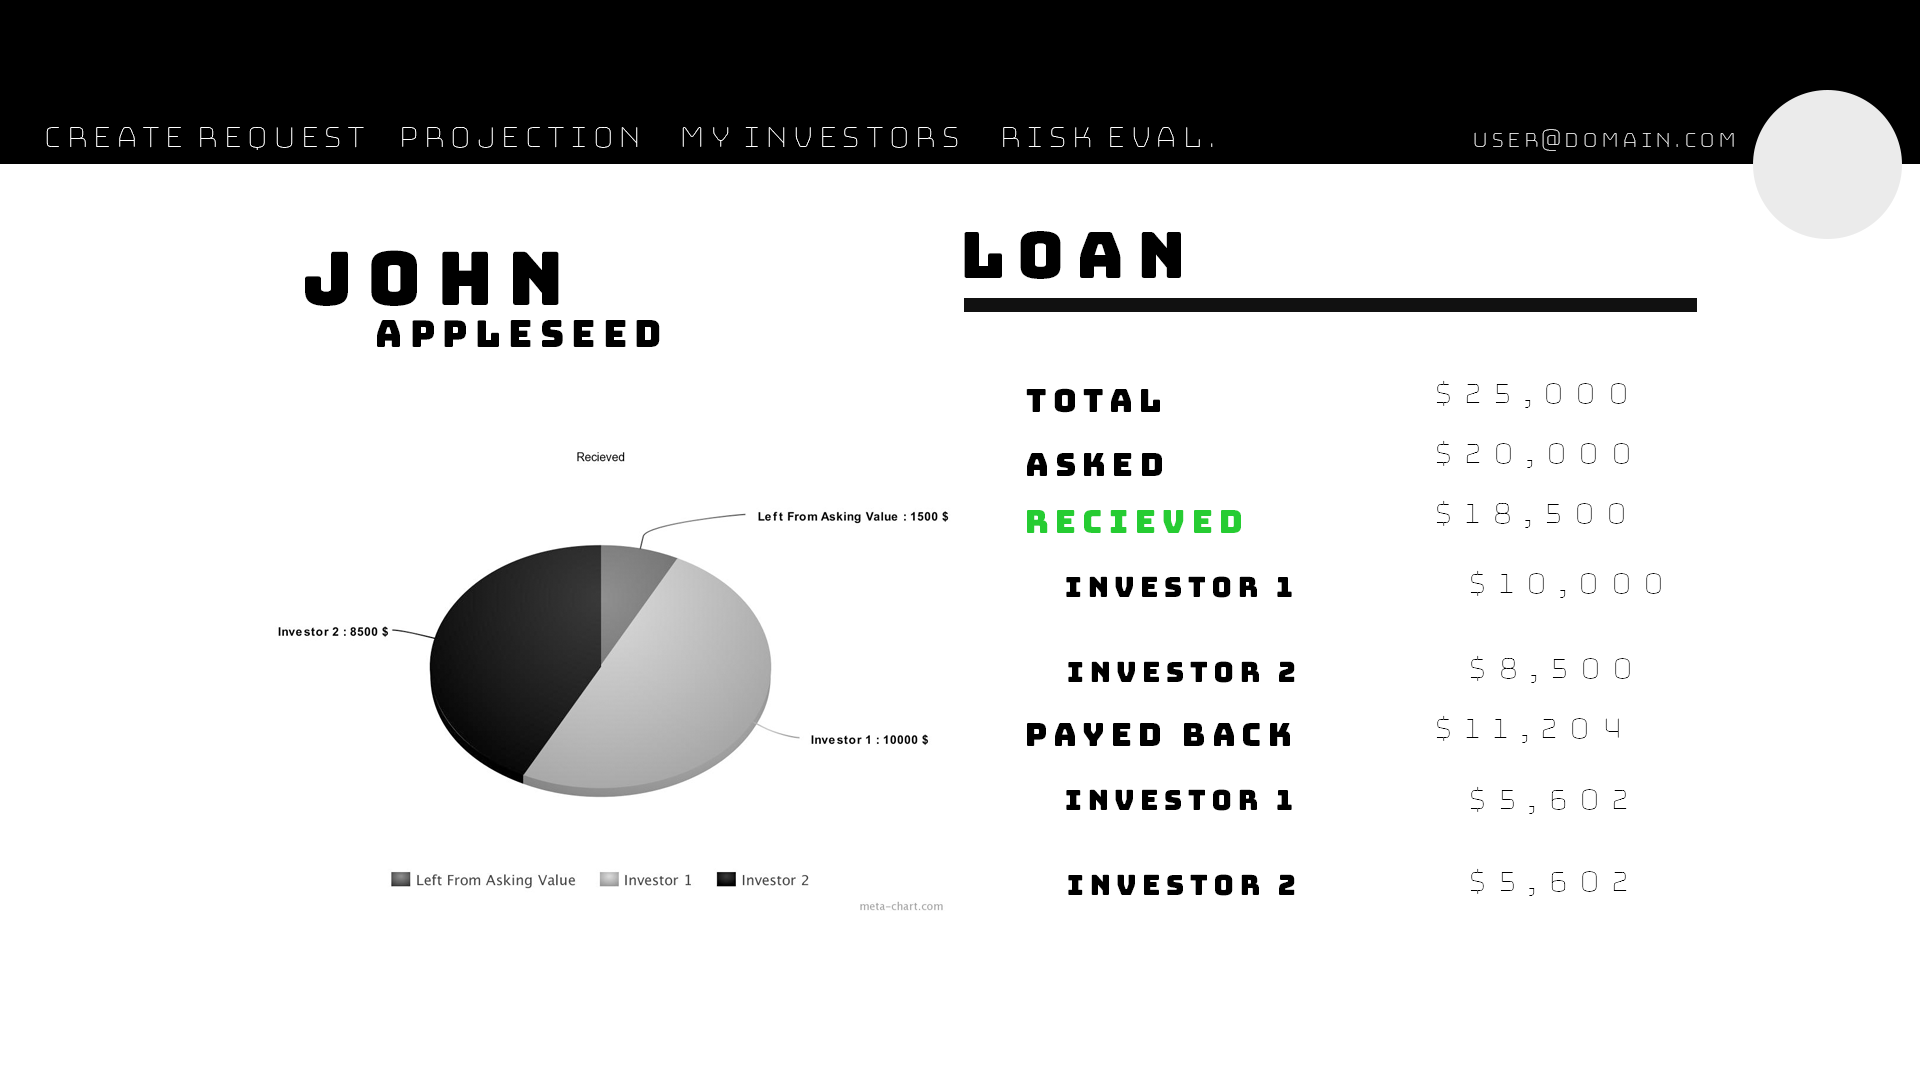
\includegraphics[width=\textwidth]{Account_Overview_Borrower}
\caption{Profile overview page}
\end{figure}


\subsubsection{UI Instructions}

\begin{enumerate}
	\item The user enters the website as a Borrower or as a Lender 
	\item Both Borrowers and Lenders enter their name and address(Figs 5,6)
	\item Borrowers enter information on the loan they wish for help with(Fig. 7); Lenders enter banking information(Fig. 8)
	\item They enter an email and password to use to login(Fig. 9), then are brought to their profile(Fig. 10)
	
\end{enumerate}